\cleartooddpage[\thispagestyle{empty}]
\chapter{Introduction}\label{CHAPTER1}

Subarachnoid hemorrhage is a potentially devastating pathologic condition in which bleeding occurs into the space surrounding the brain. One of the prevalent events that result in subarachnoid hemorrhage is the rupture of an intracranial aneurysm (IA). IAs are degenerative, irregular expansions of areas in the cerebral vasculature that occur in an estimated 3-5\% of the global population \cite{revilla2018prevalence,hackenberg2018unruptured,villablanca2013natural}, with an estimated 0.15\% - 0.7\% of the global population suffering the rupture of an IA each year \cite{hughes2018estimating}. Mortality rates due to the rupture of IAs are estimated between 45-50\%, with survivors suffering significant neurological damage, including physical and cognitive impairment \cite{LONGO2017632,villablanca2013natural}. Yet the disparity between the number of ruptured and unruptured IAs indicate that not all IAs are at high rupture risk. 
	From a clinical perspective, improved medical imaging techniques have led to an increase in the detection of unruptured IAs, and novel surgical intervention methods have aimed to reduce the instances of IA rupture and their subsequent impacts of patient health \cite{molyneux2002international,komotar2008guidelines}. Yet surgical treatments are not without a high healthcare costs: surgical repair (without complications) if IAs can be an estimated \$25,000. Data has also shown that, while treatment risks are relatively low, similar outcomes of morbidity and mortality can occur in the event of treatment complications \cite{mascitelli2015predictors,liu2016recanalization,chalouhi2015safety}. Surgical complications also result in a marked increase in costs: between \$36,188 and \$68,165 depending on possible complications (varies with surgical intervention) \cite{brinjikji2012hospitalization}. Additionally, continued economic burden is placed upon patients and their families if long term rehabilitation, home care, or in-hospital treatment is required, post-surgical complications. Therefore, elucidating the processes and conditions which impact IA rupture are of significant interest for risk stratification, improved patient selection and treatment planning.
	
Research has shown that a wide array of risk factors may impact IA development, growth and rupture potential \cite{Korja2014,penn2014role,starke2014tumor,diagbouga2018role}, but these factors can generally be broken down into three categories:
	\begin{itemize}
  		\item[--] IA morphological characteristics
 	    \item[--] Vascular hemodynamics
 	    \item[--] Patient genetic and health factors
	\end{itemize}

\subsection{Morphological Characteristics}

Morphological characteristics of IAs are oft-considered when determining rupture potential. Factors such as IA size (volume), shape, aspect ratio, IA to parent vessel angles, etc. \textcolor{red}{NEEEEED REFERENCES} have been identified in a number of studies as a possible metric to assess IA rupture potential. However, many of these parameters have been shown to generate conflicting results between studies, varying in the strengths toward rupture prediction. As per example, IAs $>$7mm in size are often associated with rupture risk, with IAs $>$25mm thought to be at the greatest rupture risk. If applied clinically, this would leave many small IAs ($<$7mm) under-treated due to the thought that the risk of complications from surgical interventions may be of greater risk than the possibility of small IA rupture \textbf{(IS THIS TRUE)}. Yet small aneurysms have been shown to be at a non-insignificant risk of rupture \cite{duan2018morphological} and not all large IAs rupture. The strength of IA size on rupture impact may be further complicated by IA location, which has also been noted to potentially impact IA rupture \cite{ucas2012natrual,weir2002sizes}. Similar to IA size, additional morphological characteristics are applied to clinical assessment of IAs, yet similar discrepancies exist between studies assessing their impact on rupture prediction.

\subsection{Hemodynamic Characteristics}

Hemodynamic stressors are thought to play a significant role on the initiation, growth and possible rupture of IAs. Tangental fluid stressors along the vascular wall, known as wall shear stress (WSS), and its derivatives are often of investigated when generating models for IA rupture prediction(s)\cite{Jing2015,Xiang2011WSS,doddasomayajula2017hemodynamic,Cebral510}. These near-wall forces have been shown to act as a biological stimulator, eliciting various changes to both vasculature endothellial and smooth muscle cells, inducing changes in gene expression, phenotypical and mechanical properties, and protein expressions which dictate cellular activity \cite{baek2009flow,van2010analyzing,dolan2013high,sato2000local,baeyens2016endothelial,byrne2014quantifying,cecchi2011role,kulcsar2011hemodynamics}. While likely triggers to vascular cell changes, discrepancies exist, similar to IA morphological characteristics, of to which specific hemodynamic characteristics impact IA rupture prediction and their overall predictive strength. It has been shown that vascular cells maintain healthy physiological characteristics while exposed to a range of WSS between 3 and 15 dynes/cm$^{2}$ yet studies are in conflict if WSS lower \cite{Miura519,boussel2008aneurysm} or higher \cite{dolan2013high,shojima2004magnitude} from said preferred range is of greater impact on IA rupture risk. It has been suggested that both high and low WSS trigger differing impacts on vascular cells \cite{Meng1254} which both may play a significant role in IA development and potential rupture. Even focusing on one extrema of WSS values and determining their usefulness on prediction IA rupture risk has proven difficult. In a 2016 meta analysis by Zhou, the impact of low wall shear stress on predicting IA rupture varied between studies (Fig.~\ref{Low_WSS_meta_analysis}). Nonetheless, while the exact role of WSS and its impact on IA rupture is still being elucidated, WSS if often applied to a number of studies aiming to determine the characteristics of IAs a high risk of rupture. It is worth noting, that the clinical measurement of hemodynamic characteristics and WSS \textit{in-vivo} is possible, yet remains difficult especially in smaller blood vessels and small IAs. Improvements in computational fluid dynamics (CFD) can help overcome the limitations of \textit{in-vivo} WSS measurement and is being adopted as a clinical tool for assessment of rupture potential and planning of IA treatments \cite{steinman2002image,valen2013mind}. 

\begin{figure}[!h]
\begin{center}
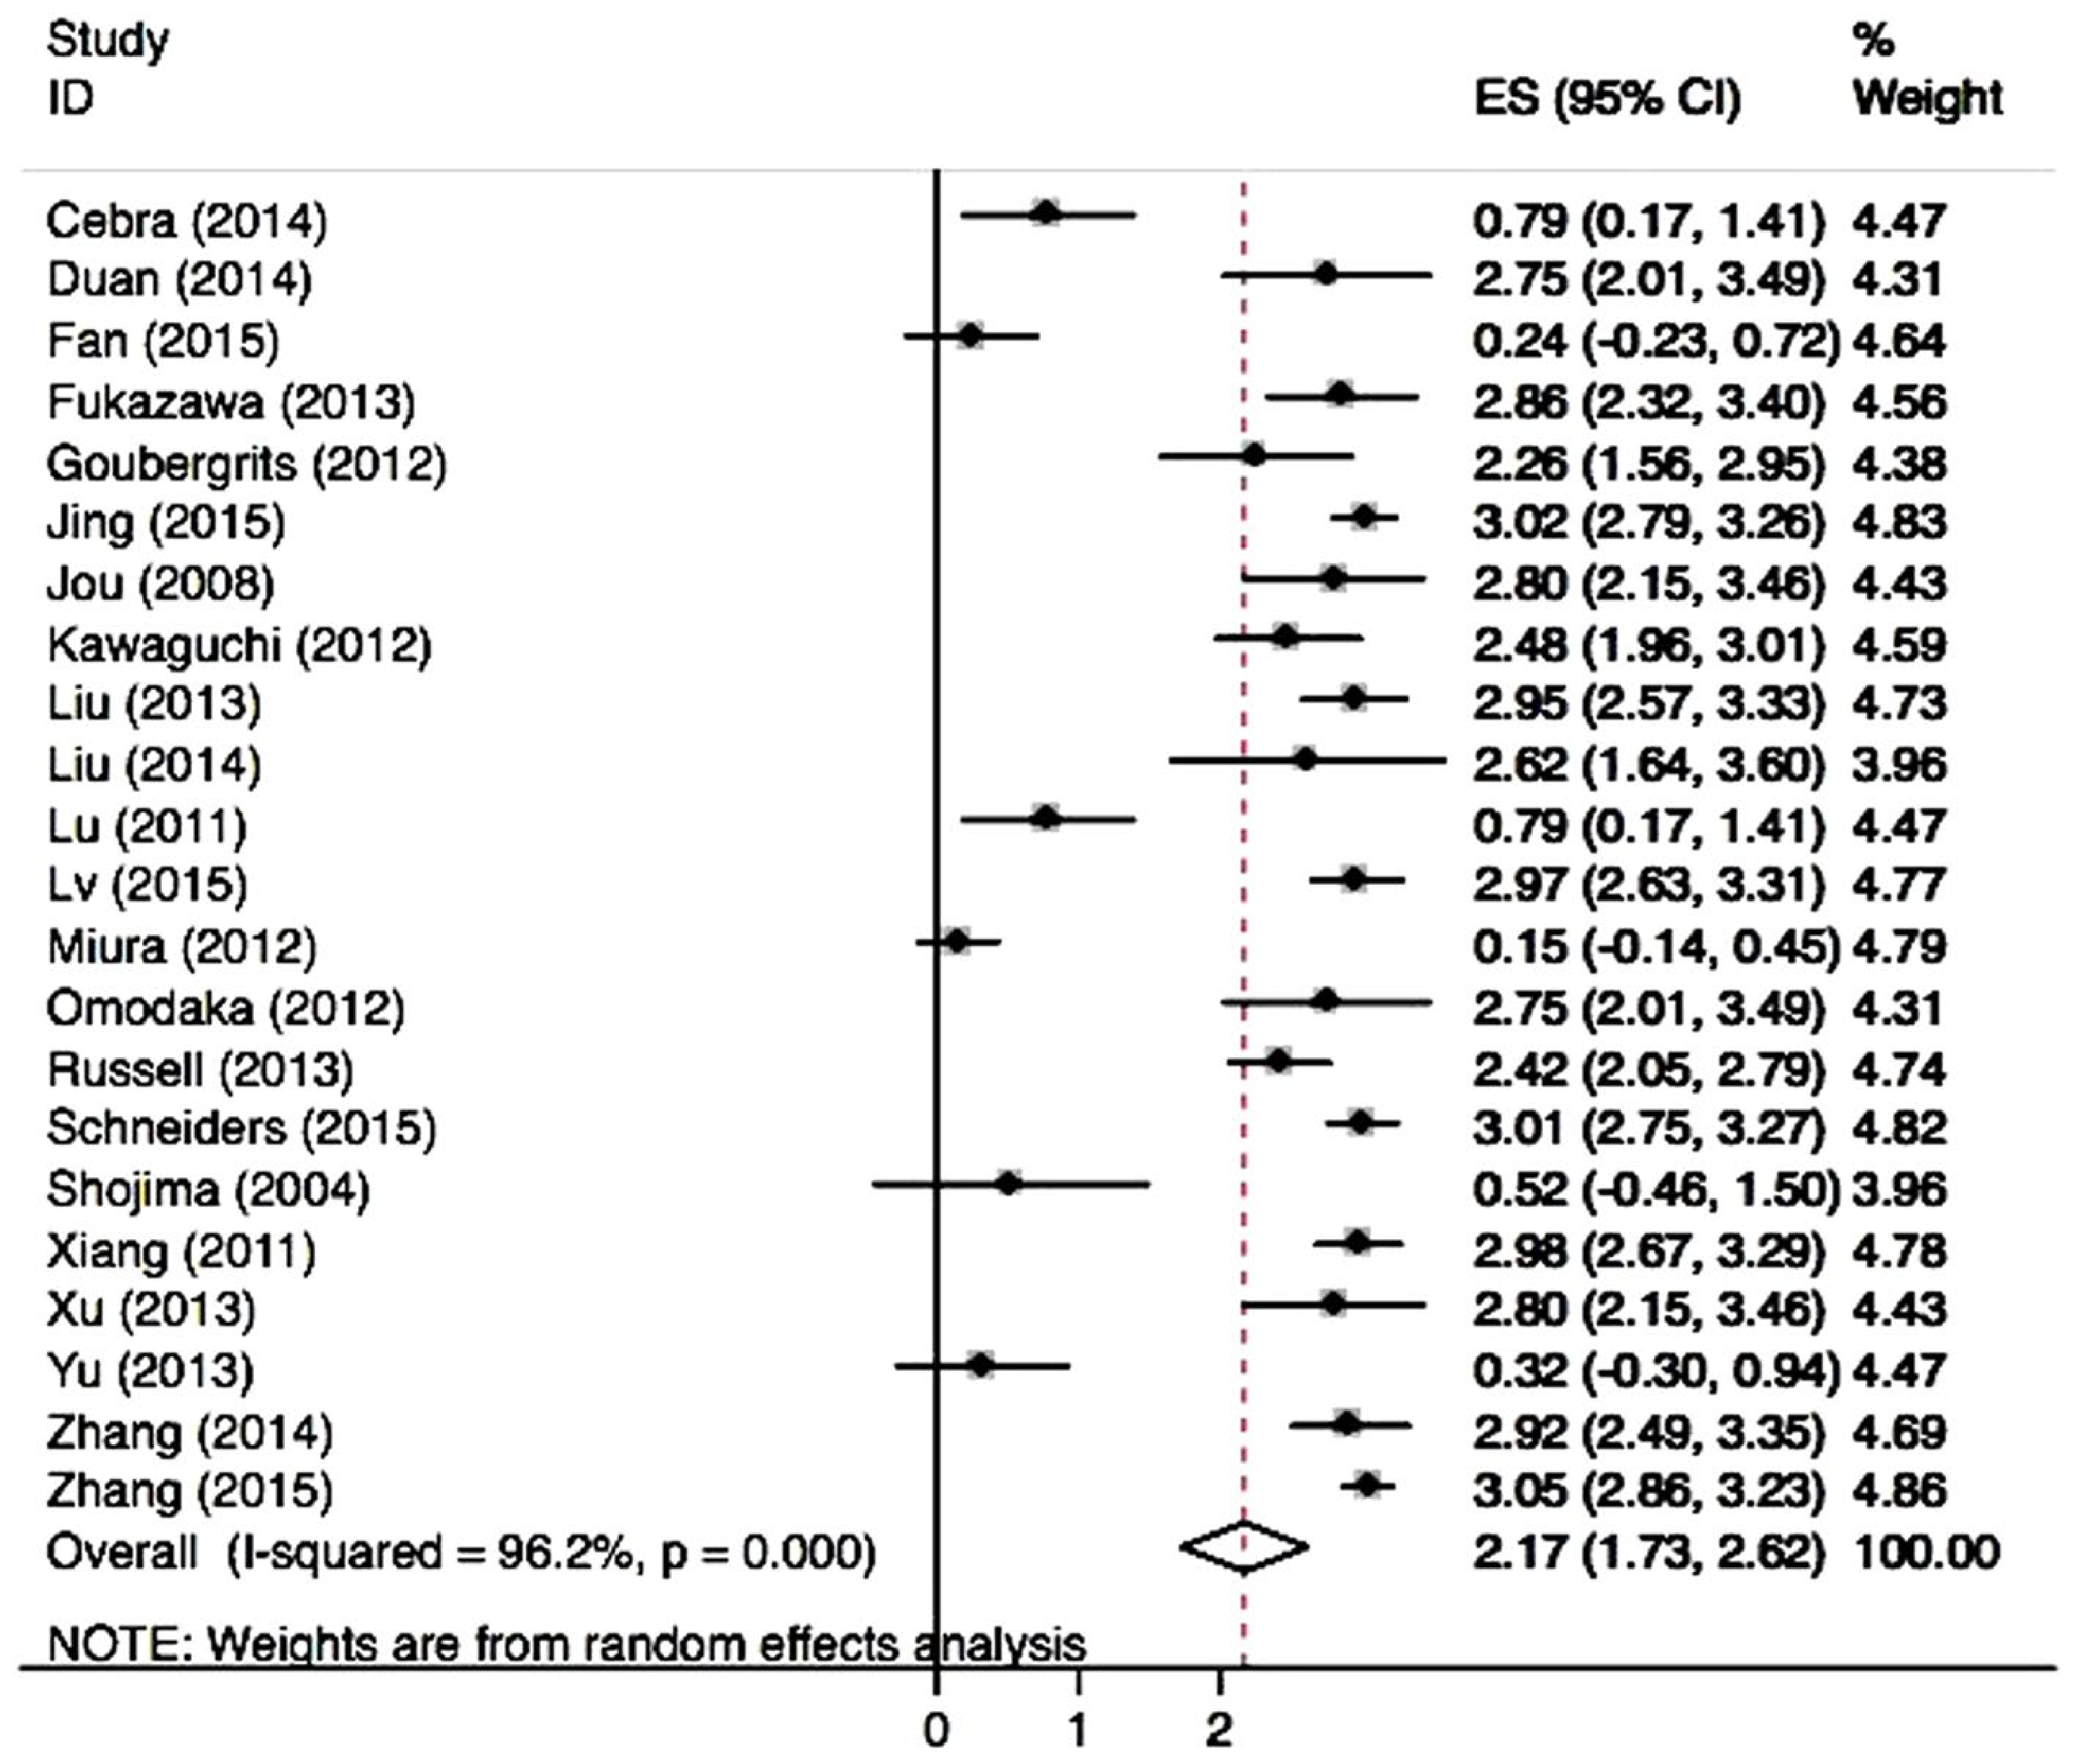
\includegraphics[width=3.34in]{Zhou_2016_Meta_analysis_low_WSS_fig1.eps}
\captionsetup{width=0.5\textwidth, justification=justified,singlelinecheck=false}
\caption{Zhou 2016 Meta-analysis of the reported low WSS rate of rupture aneurysms and the Odds Ratio for low WSS in predictive modeling}
\end{center}
\label{Low_WSS_meta_analysis}
\end{figure}


While a number of metrics (geometric, hemodynamic, and health factors) have aided in understanding possible mechanisms triggering IA development and rupture, these aforementioned metrics overlook the broader flow patterns occurring within the aneurysm sac and parent vessel. Initial investigations into areas of likely IA development correlated their development with areas of high vessel curvature or at areas of vessel bifurcation. These specific vascular geometries can generate irregular swirling flow patterns (vortices) which were hypothesized to impact IA development and rupture. Investigations of hemodynamic vortices in both \textit{in-vivo} and \textit{in-vivo} and have been shown to elicit endothelial cell dysfunction \cite{balaguru2016disturbed,mannino2015yourself,nowicki2014novel}.

%Current surgical interventions typically focus on occluding blood flow into an IA. IA clipping involves opening the skull to place a titanium clip around the opening (ostium) of the IA. Yet a meta-analysis between 1990 and 2011 showed this surgical methodology carried with it a 1.7\% and 6.7\% mortality and morbidity rate (respectively) \cite{Kotowski42}. A more recent method to repair IAs and prevent their potential rupture is through coiling: the implantation of flexible platinum wires inside an IA to create an artificial thrombosis within the IA sac. A combination of coiling alongside implantation of a stent across the IA ostium may be used to help ensure proper coil retention within the IA sac. Treatment of IAs with coiling has been shown to have an 80-85\% success rate \cite{molyneux2002international}, yet carries with it complication risks: morbidity, mortality, coil slippage, incomplete occlusion or coil compaction \cite{hoppe2015comparison,liu2016recanalization}. While clinical intervention methods have been shown to reduce the onset of IA rupture, they are not without their own inherent physiological risk, leading to similar neurological damage as a ruptured IA\cite{liu2016recanalization,mascitelli2015predictors,chalouhi2015safety}.

Typically, the geometrical properties of IA and their surrounding vasculature as well as patient medical history and health factors (smoking, diabetus, etc) \cite{Backes951} have been linked with IA rupture. \cite{Steiner_2018,Thompson2015guidelines}. Additionally, a growing body of research has focused on the hemodynamic stressors along the IA wall, and how they may contribute to the development of IAs and their and potential rupture, specifically how they trigger pathologic changes to vascular cells \cite{baek2009flow,dolan2013high,byrne2014quantifying,cecchi2011role,kulcsar2011hemodynamics}. 


To better differentiate aneurysms at risk of rupture, novel assessment of the ever-chaining hemodynamic conditions within the IA sac may hold they key. Flow patterns within aneurysm, specifically the swirling flow (vortices) in IAs, have been thought to impart pathologic cellular changes to vascular cells. Yet the presence of swirling flow patterns, or a visual, qualitative appraisal of flow complexity is what is typically correlated with IA rupture risk. The focus of this thesis is that by applying a novel analysis technique to assess the temporal changes to vortices' stability and complexity over the cardiac cycle and how they may be useful in identifying the possible development and rupture potential of cerebral IAs. 



Lorem ipsum dolor sit amet, at qui viderer recusabo aliquando, dignissim 
evertitur ei his. Ignota iuvaret fabulas ei vim. Ne utinam inciderint quo. 
Pri ea congue postulant conclusionemque. Ut elitr dicam elaboraret pro, ius 
altera voluptaria cu. Eam mazim aliquip cu, recusabo pericula accommodare at 
mea, facer affert nonumes qui ea.

Discere dissentiet vel et, soluta nostrum epicurei ad eam, cu has aperiam 
vituperata. In prima quaeque diceret pri. Enim labores contentiones eos at, 
duo altera denique nominavi ea, eos inani nominavi consectetuer at. Ut elitr 
dicam elaboraret pro, ius altera voluptaria cu. Eam mazim aliquip cu, 
recusabo pericula accommodare at mea, facer affert nonumes qui ea.
\cite{Crystal09_01,DMOL3_01,HPL_DGEMM_02}

\section{Section 1}\label{CHAPTER1_SECTION1}

At vix indoctum disputando. Eam cu doctus reprimique, quaeque democritum 
an eos, sit veniam facete dissentias id. Tale volumus eos te, an eum nulla 
tincidunt. Mea id recteque theophrastus.

Eirmod malorum vis ei. Choro euismod incorrupte in vim, ludus ornatus vis ex. 
Hinc wisi impedit eum no, vocent definiebas referrentur in quo. Sanctus 
vulputate repudiandae usu ut.

\subsection{Objective}\label{CHAPTER1_SECTION1_SUBSECTION1}

Although there exists a number of studies\cite{can2015association,zhou2017association,varble2018stroke} and methodologies\cite{etminan2015unruptured,greving2014development} that attempt to assess IAs at a high risk of rupture, inconsistencies between study outcomes leave the development of an ideal predictive model out of reach. In addition, many of these previous studies assess the geometric\cite{abboud2017morphology,kashiwazaki2013size,varble2018stroke} and/or hemodynamic wall stressors\cite{zhou2017association,Miura519,can2015association} as a means to predict IA rupture, with limited quantitative assessment of the hemodynamic flow conditions within the aneurysm. \textbf{The primary objective} of this work is to assess the viability of adapting quantitative analysis of hemodynamic flow patterns, specifically swirling flow pattern(s) (vortex), within IAs to improve the prediction and understanding of IA rupture. In this work, an overview of recent theories concerning 

\begin{figure}[htb]
  \begin{center}
    \begin{tikzpicture}[scale=0.60, every node/.style={scale=0.60}]
      \path[mindmap,concept color=Black,text=White]
      node[concept] {\begin{equation*}\sum_{i,j=1}^{M,N}\,\alpha_{ij}\,\beta_{ji}\,=\,?\end{equation*}}
      [clockwise from=0]
      child[concept color=RoyalBlue!65!Black] { node[concept] {A1}
        [clockwise from=90]
        child { node[concept] {ABCD} }
        child { node[concept] {EFGH} }
        child { node[concept] {IJKL} }
      }
      child[concept color=OrangeRed!65!Black] { node[concept] {B2}
        [clockwise from=0]
        child { node[concept] {TUVWX} }
        child { node[concept] {YZABC} }
      }
      child[concept color=DarkGoldenRod!65!Black] { node[concept] {C3}
        [clockwise from=-45]
        child { node[concept] {123} }
        child { node[concept] {789} }
      }
      child[concept color=Plum!65!Black] { node[concept] {D4}
        [clockwise from=-90]
        child { node[concept] {$\alpha$} }
        child { node[concept] {$\beta\,\gamma$} }
        child { node[concept] {$\pi$} }
        child { node[concept] {$\eta$} }
      }
      child[concept color=ForestGreen!65!Black] { node[concept] {$\nabla\,\psi \,=\, \delta\,\phi$}
      }
      child[concept color=LightCoral!65!Black] { node[concept] {\begin{equation*}\int_{0}^{\infty}\,\frac{1}{x}\,dx\end{equation*}}
      } ;
    \end{tikzpicture}
  \end{center}
  \caption{Schematic representation of our universe}
  \label{CHAPTER1_FIG01}
\end{figure}


\subsection{Methodolgy}\label{CHAPTER1_SECTION1_SUBSECTION2}
For the initial focus of this work, image-based computational fluid dynamics models of patient-specific IA geometry will be constructed from 3D phase contrast magnetic resonance imaging (PC-MRI). Computational fluid dynamic (CFD) simulations will be performed on the computational models to generate realistic 3D hemodyanmic velocity and flow pattern data. From said data, 


\begin{figure}[htb]
  \begin{center}
    \begin{tikzpicture}[domain=0:4]
      \draw[very thin,color=gray] (-0.1,-1.1) grid (3.9,3.9);
      \draw[->] (-0.2,0) -- (4.2,0) node[right] {$x$};
      \draw[->] (0,-1.2) -- (0,4.2) node[above] {$f(x)$};
      \draw[color=red] plot[id=x] function{x}
        node[right] {$x$};
      \draw[color=blue] plot[id=sin] function{sin(x)}
        node[right] {$\sin x$};
      \draw[color=orange] plot[id=exp] function{0.05*exp(x)}
        node[right] {$\frac{1}{20} \mathrm e^x$};
    \end{tikzpicture}
  \end{center}
  \caption{Mathematical functions plotted using TikZ package}
  \label{CHAPTER1_FIG02}
\end{figure}

Simul noster voluptaria eam ei, sint regione pri ei. Cum no utinam equidem, 
falli bonorum prodesset an qui. Alterum dissentiet vituperatoribus te eam, 
eos ea suas oblique. Per ea utinam facilisi. \cite{DMOL3_02,HPL_01,HPL_02}
Per iudico probatus complectitur et, cum tollit atomorum rationibus ea.

\section{Aneurysm Geometic Characterisitcs}\label{CHAPTER1_SECTION2}

All aneurysm geometries were taken from the finalized computational mesh generated for simulations. The aneurysm sac was manually isolated from the parent vessel and the resultant cut plane was capped and identified as the IA ostium using an in-house script written in VMTK. Geometric measurements were either taken directly from the values reported in the Aneurisk dataset, or were calculated using in-house scripts in VMTK. 

\underline{Aneurysm Surface Area and Volume}: Measured directly from the isolated IA geometry before and after (respectively) ostium capping. A number of studies have eluded to an increase in IA size as a risk for both IA growth and rupture. \cite{varble2018stroke,brinjikji2015risk,Backes951,greving2014development}. A meta-analysis performed by Brinjikji et al reported that IA $\le$ 10 mm in size (diameter) grew at a rate $<$ 2.9\% per year, while IAs $>$ 10 mm were associated with growth rates of 9.7\% per year. This growth was also reported with an associated IA rupture rate: 3.1\% per year compared with 0.1\% per year for stable (non-growing) aneurysms (p $\le$ 01). From a clinical perspective, the overall size of an aneurysm is often a characteristic used to determine course of IA treatment (or lack thereof) \cite{williams2013management,komotar2008guidelines}. Yet while large IAs are thought to increase the likelihood of rupture, a not-insignificant number of small IAs ($<$5 mm diameter) also have been shown to rupture \cite{kashiwazaki2013size,forget2001review,Korja2014}. This disparity between sizes of ruptured IAs suggest that the assessment of additional factors in tandem with IA size may improve rupture prediction. 

\underline{Aneurysm Height}: The length of the centerline of the IA sac is measured, following the IA shape, as opposed to measuring a straight line from the ostium centroid directly to the highest IA point. The radius of the maximum inscribed sphere at the centerline's furthest point is added to the length measurement to fully measure the IA height. This is a modified version of the typical IA height measurement: a straight line of the maximum stretch from the ostium centroid to the IA dome \cite{ma2010size,duan2018morphological}. 

\underline{Vessel Diameter}: The parent artery diameter value is computed at locations close to the aneurysm ostium. For terminal aneurysms, the vessel diameter of the common branch was measured at the point prior to centerline splitting between the daughter arteries, and both daughter arteries' diameter were measured at the point one (common artery) diameter away from the IA ostium cut. The average of the three values was used as the value of the vessel diameter.

\underline{Inlet Cross-sectional Area}: The beginning of the inlet vessel was cut square in the 3-matic software package, the resultant cross-sectional area of the inlet vessel was calculated. 
 
\underline{Aspect Ratio$^*$}: A modified calculation of the commonly defined aspect ratio (aneurysm hight/ostium diameter) was used by adapting the length of the centerline of an IA as the IA height (IA$_{height^*}$), and the area and circumference of the ostium since ostium diameter is rarely uniform for an IA \cite{piccinelli2012characterization}.
\begin{equation}
Aspect Ratio^* = \frac{IA_{height^*}}{4*(Ostium_{area} / Ostium_{circumfrence})}
\end{equation}

The aspect ratio of an IA has been shown to be correlated with levels of hemodynamic stressors and has been used as an ease-of-use method to assess conditions within an IA \cite{zeng2011can}.  

\section{Aneurysm Hemodynamic Characterisitcs}\label{CHAPTER1_SECTION3}


\underline{Wall Shear Stress}: 
The calculation of wall shear stress (WSS) is performed by the ANSYS-FLUENT commercial finite-element solver (ANSYS v17.0). The value is defined as the normal velocity gradient against the (vessel) wall:
\begin{equation} \label{WSS}
\tau_w = \mu\frac{\partial v}{\partial n}
\end{equation}
with $\mu$ as the fluid dynamic viscosity (0.004 kg/m-s). 

The spatial-temporally averaged value of the aneurysm's WSS was calculated alongside its temporally-averaged WSS minimum and temporally-averaged WSS maximum. In a similar manner as IA volume, research differs on wither high \cite{dolan2013high} or low \cite{Zhang2016} wall shear stress is a better predictive metric for IA rupture potential. In a study by Meng et. al., both high and low WSS were associated with IA rupture potential, yet causing differing cellular changes \cite{Meng1254}. 

\underline{Kinetic Energy Density}:
The kinetic energy density (KED) within the IA dome was calculated as follows:
		\begin{equation}
KED = \frac{\frac{1}{2}\rho\sum v^2}{n}
	\end{equation}
Where $v$ is the velocity values, $\rho$ is the mass density of blood, and $n$ is the number of voxels within the IA. The KED at each time-step (along the cardiac phase) was calculated, as well as the Temporally averaged KED (TA-KED) for all cases. 

\section{Disturbed Flow on Vascular Endothelium}\label{Chapter1_Section4}

The vascular endothelial cell (EC) layer forms the innermost lining of blood vessels, directly interacting with hemodynamic stressors and helping to maintain homeostatic functions of the vasculature\cite{chien2007mechanotransduction,gimbrone2016endothelial}. The mechanotransduction capabilities of this initial vascular layer help maintain a selective macromoleuclar barrier, trigger vascular remodeling, regulate vascular smooth muscle cell contraction\cite{vanhoutte2009endothelial}, and help control vascular inflammatory responses\cite{chalouhi2012biology}. The degradation of vascular homeostatsis, resultant from disturbed hemodynamic flow patterns, has been associated with an array of vascular pathologies: aneurysms\cite{Cebral119,LONGO2017632}, atherosclerosis\cite{Liu2015}, and thrombosis\cite{chiu2011effects,uzarski2013adaptation}. Due to the life threating nature of IAs, improved quantitative methods to characterize hemodynamic patterns and to what degree they impart EC pathologic changes, could prove essential to further our understanding of the disease's initiation and progression. 

The morphology and cytoskeletoal organization of EC have been shown to be susceptible to non-laminar flow conditions\cite{wang2013endothelial}. Typically, EC morphology aligns along flow directionality, forming organized parallel actin stress fibers and giving the cells an elongated  
structure\cite{thomas2016biomimetic,gimbrone2016endothelial,balaguru2016disturbed}. Disrupted flow patterns resulting in vortex flow and altered WSS, show a differential change in EC characteristics: a rounded morphology with marginally located short actin stress fibers\cite{chiu2011effects,uzarski2013adaptation,dolan2011high}. These changes have been associated with a number of structural-fucntional changes in vasuclar cells, such as increased permeability to macromolecules, increased expression of adhesion molecules (ICAM-1, VCAM-1), decreased endothelial cell regeneration and increased smooth muscle cell proliferation/migration.


Additionally, inflammatory processes within vasculature has been shown to be a significant actor in the pathogenesis of IA development and potential rupture \cite{chalouhi2012biology,hashimoto2006,signorelli2018}. In a typical physiological setting, the vascular EC layer maintains antiatherogenic characteristics, inhibiting platelet adhesion and aggregation along the vascular wall, as well as limiting cellular pro-inflammatory pathways\cite{ALSOUDI2017951}. In the occurrence of IA pathology, a breakdown of the EC inflammatory-limiting capabilities is noted: small aneurysm shown to have intimal thickening and diffuse macrophage/lymphocyte infiltration, whereas chronic atherosclerotic lesions with embedded macrophages and lymphocytes have been noted in larger aneurysms\cite{Frösen2012,kosierkiewicz1994}. Upon leukocyte and macrophage infiltration, the matrix metalloproteinase enzyme is released which digests extracellular matrix proteins leading to additional pathologic damage to the vascular wall\cite{tronic2000,aoki2007a}. The remodeling of the vascular wall, impart due to inflammatory pathogenic activities, lead to an overall loss vessel mechanical strength and a possible ballooning out of the impacted area   



Docendi eligendi sit et, pri ea dicam eligendi percipitur, has soleat 
dolores convenire te. Sed altera placerat an, id verterem abhorreant 
interesset mea. Eum at ceteros efficiantur. Eos id voluptaria efficiendi 
comprehensam. \cite{HPL_DGEMM_01,HPL_DGEMM_02}

\begin{figure}[hbt]
  \begin{center}
    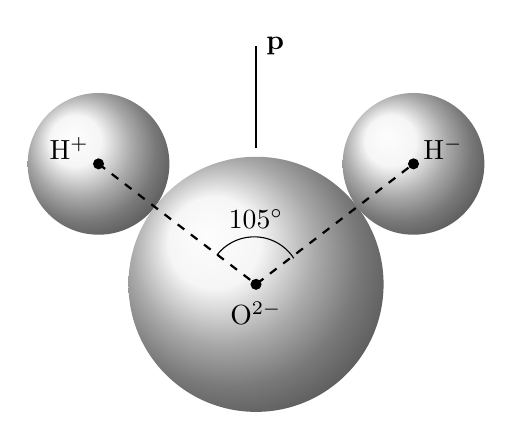
\begin{tikzpicture}[>=latex,scale=1.0]
      \shade[ball color=gray!10!] (0,0) coordinate(Hp) circle (.9) ;
      \shade[ball color=gray!10!] (2,-1.53) coordinate(O) circle (1.62) ;
      \shade[ball color=gray!10!] (4,0) coordinate(Hm) circle (.9) ;
      \draw[thick,dashed] (0,0) -- (2,-1.53) -- (4,0) ;
      \draw[thick] (2,.2) -- (2,1.5) node[right]{$\mathbf{p}$} ;
      \draw (2.48,-1.2) arc (33:142:.6)  ;
      \draw (2,-.95) node[above]{$105^{\circ}$} ;
      \draw (0,.2) node[left]{H$^+$} ;
      \draw (4,.2) node[right]{H$^-$} ;
      \draw (2,-1.63) node[below]{O$^{2-}$} ;
      \foreach \point in {O,Hp,Hm}
        \fill [black] (\point) circle (2pt) ;
    \end{tikzpicture}
  \end{center}
  \caption{Schematic representation of a water molecule}
  \label{CHAPTER1_FIG03}
\end{figure}

In mel modo dicam vocibus, eruditi consectetuer vim no, cu quaestio 
instructior eum. Justo nostrud fuisset ea mea, eam an libris repudiandae 
vituperatoribus. Est choro corrumpit definitionem at. Vel sint adhuc vocibus 
ea, illud epicuri eos no. Sea simul officiis ea, et qui veri invidunt 
appellantur. Vix et eros ancillae pertinax. 
\cite{GROMACS4,GULP_01,GULP_02,HYPRE_01,LAMMPS_01}
Per iudico probatus complectitur et, cum tollit atomorum rationibus ea.
Per iudico probatus complectitur et, cum tollit atomorum rationibus ea.

Aliquip lobortis ei est, at error viris graeco sed. Vel te elitr detracto, 
modo graecis scripserit ex nec. Errem utamur viderer per no, eam ea eripuit 
referrentur. Pro te dicat disputando. Per iudico probatus complectitur et, 
cum tollit atomorum rationibus ea. \cite{R_01,SIESTA_01,SIESTA_02,SMEAGOL_01}.
Per iudico probatus complectitur et, cum tollit atomorum rationibus ea.

Per iudico probatus complectitur et, cum tollit atomorum rationibus ea.
Docendi eligendi sit et, pri ea dicam eligendi percipitur, has soleat 
dolores convenire te. Per iudico probatus complectitur et, cum tollit 
atomorum rationibus ea.
